% \documentclass[11pt]{article}
\documentclass[aps,chaos,superscriptaddress,showkeys]{revtex4}
\usepackage{amsfonts,amssymb,amsmath,latexsym,epsfig,enumerate,color}

\begin{document}

\begin{center}
\section*{ \Large {Response to the referees and summary of changes} }
Date: {\today}
\end{center}

\noindent Dear editor,

\vspace{0.6cm}
We would like to resubmit our revised manuscript entitled \\

\noindent {\bf Ordinal partition transition network based complexity measures for inferring coupling direction and delay from time series } \\

\noindent by Y. J. Ruan, R.V. Donner, S. G. Guan, and Y. Zou, \\

\noindent originally submitted for publication to \emph{Chaos} with the manuscript number {\bf \#181384}.

\vspace{0.6cm}
Thank you very much for the comments and suggestions of the two
referees. All these comments helped us to improve the manuscript. We have
marked all changes in the manuscript in red color to facilitate the reading.

\vspace{0.6cm}

Please find below a detailed response to all specific remarks and questions
raised by the referees. We hope that our revised manuscript is now acceptable for
publication in \emph{Chaos}.

\vspace{0.6cm}
\noindent
Sincerely yours,\\

\vspace{0.1cm}
\noindent
Y. J. Ruan, R.V. Donner, S. G. Guan, and Y. Zou


\newpage
\begin{center}
{\bf Response to the first referee}
\end{center}


{\sf The authors are claiming to have proposed three measures for inferring coupling directions and delays from time series based on ordinal patterns. The first one, based on the standard deviation for conditional probabilities, might be new. But, the second one and the third one have been defined previously as far as I searched: The second one seems to be used at least in Li and Ouyang, NeuroImage 52, 497 (2010), while the third one was used in Staniek and Lehnertz, Phys. Rev. Lett. 100 158101 (2008). Thus, the novelty for the manuscript should be compromised and the authors should cite these preceding papers and allocating their contribution in the existing literature more appropriately. Their results shown in the figures look promising. Especially, the coupling direction and delay for the daily surface air temperature record from Oxford to that of Vienna sound reasonable. Therefore, the authors should give the credits for the related previous papers properly for the publication in Chaos. }


\begin{center}
\begin{minipage}[c]{0.9\textwidth}
We thank the referee for pointing these references, which have been properly cited in the revision. We agree that our measures have much similarities with those that have been pointed by the referee, but the same time, we wish to emphasize the difference as follows: 

The second complexity measure $H_{X \to Y}(\tau)$. 


The third complexity measure KLD indeed shows much similarity with the symbolic transfer entropy as proposed by Staniek and Lehnertz. However, there is much difference with the choice of parameter $\tau$. In the reference of Staniek et al, $\tau$ is treated as an algorithmic parameter which had been suggested as $\tau = 1$. Furthermore, it has been assumed that the empirical choice of $\tau = 1$ is always applicable if a meaningful natural sampling rate of time series is a available. However, our method interprets $\tau$ differently, considering to extract the proper coupling delay $\tau$ explicitly by treating it as a dynamical unknown variable. We have included the discussion in the revision when introducing the KLD complexity measure. 
\end{minipage}
\end{center}


\noindent
{\sf In the abstract and the main text, OPTN is defined as an abbreviation for two different phrases. In the abstract, it comes from ordinal pattern transition networks, while in the main text, it comes from ordinal partition transition networks. Please define the abbreviation by one of them. }

\begin{center}
\begin{minipage}[c]{0.9\textwidth}
In the revision, we use of the acronym for OPTN as ordinal partition transition network, which keeps the consistency with the literature. This has been corrected for both the abstract and the main text. 
\end{minipage}
\end{center}

%%%%%%%%%%%%%%%%%%%%%%%%%%%%%%%%%%%%%%%%%%%%%%%%%%%%
\vspace{0.4cm}
\begin{center}
{\bf Response to the second referee}
\end{center}


\noindent {\sf The main purpose of the manuscript is to show that ordinal pattern transition networks (OPTNs) from time series can provide an approach to improve our understanding of the underlying dynamical system (responsible for the data). The authors conclude that OPTNs can be used as complementary tools for causal inference tasks. 

The text is a well-written and scientifically sound manuscript that adds understanding to the important area of time series analysis. Before its publication, I believe some questions must be better answered by the authors. }


\begin{center}
\begin{minipage}[c]{0.9\textwidth}
We thank the referee for the overall positive evaluation on our manuscript. 
\end{minipage}
\end{center}


\noindent {\sf 1- On figures 4 - 8 and 11. The authors claim the results are "based on averages over 20 independent realizations of the considered processes". So the dispersion of the mean values (plotted by error bar or any other way) must be included. A discussion about dispersion values will bring more information about the validity of the results.  }


\begin{center}
\begin{minipage}[c]{0.9\textwidth}
This is indeed a nice comment. In the very beginning, we plan to include the error bars in all figures. However, we show in this reply letter, these error bars are really invisible even though we have magnified by 1000 times as shown in Figs. \ref{fig:stdHeqB} - \ref{fig:stdHeqE}. Later we decided not to include the error bars in the manuscript. 

\end{minipage}
\end{center}
\begin{figure}
	\centering
	\includegraphics[width=0.5\columnwidth]{/Users/yongzou/Documents/TimeSeries_Network/OrderPatternPermutation/RuanFiguresPlot2018/errorbarE_B.eps}
%	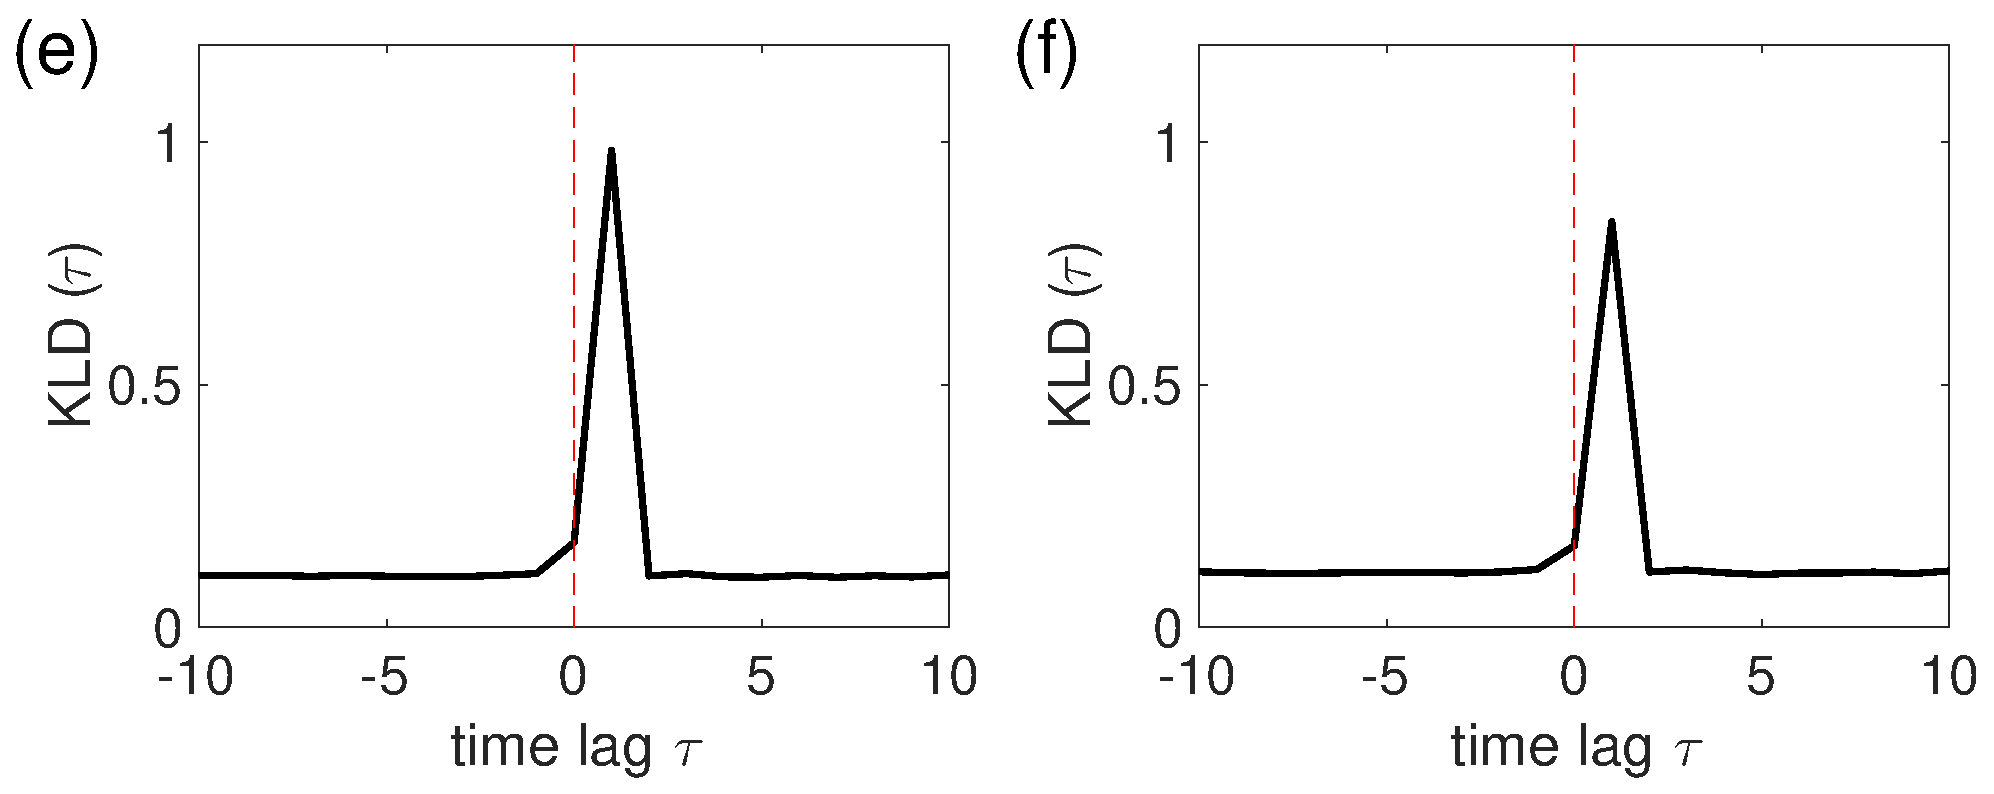
\includegraphics[width=\columnwidth]{KL_B.eps}
\caption{(Color online) Values of three ordinal pattern co-occurrence complexity measures in dependence on the mutual delay $\tau$ for realizations of Eq. (1): (a,b) $\sigma_{X\to Y}(\tau)$, (c,d) $H_{X \to Y}(\tau)$, (e,f) $\text{KLD}(\tau)$. (a,c,e) show the results for realizations from the linear model, while (b,d,f) correspond to the nonlinear transformation of the first subsystem as described in the text. The vertical red dashed lines indicate the values for vanishing mutual delay ($\tau=0$). {\color{red}Note that the error bars have been enlarged by 1000 times.} \label{fig:stdHeqB}}
\end{figure}

\begin{figure}
	\centering
	\includegraphics[width=0.5\columnwidth]{/Users/yongzou/Documents/TimeSeries_Network/OrderPatternPermutation/RuanFiguresPlot2018/errorbarE_C.eps}
%	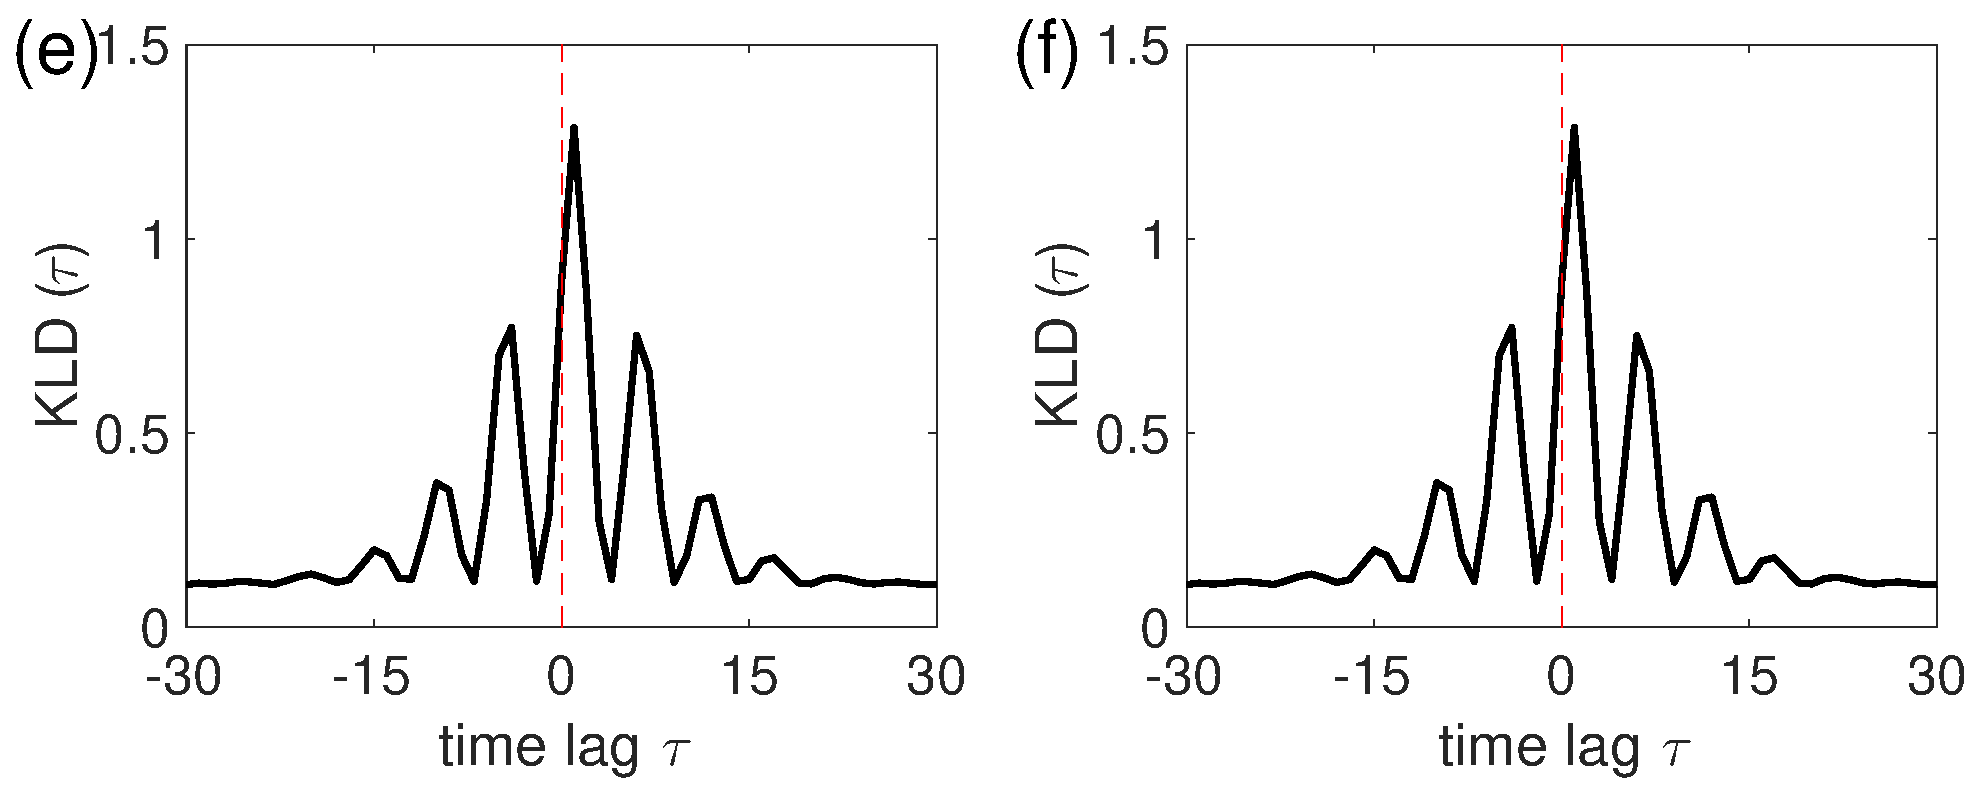
\includegraphics[width=\columnwidth]{KL_C.eps}
\caption{(Color online) Same as in Fig.~\ref{fig:stdHeqB} but for Eq. (10). {\color{red}Note that the error bars have been enlarged by 1000 times.} \label{fig:stdHeqC}}
\end{figure}

\begin{figure}
	\centering
	\includegraphics[width=0.5\columnwidth]{/Users/yongzou/Documents/TimeSeries_Network/OrderPatternPermutation/RuanFiguresPlot2018/errorbarE_D.eps}
%	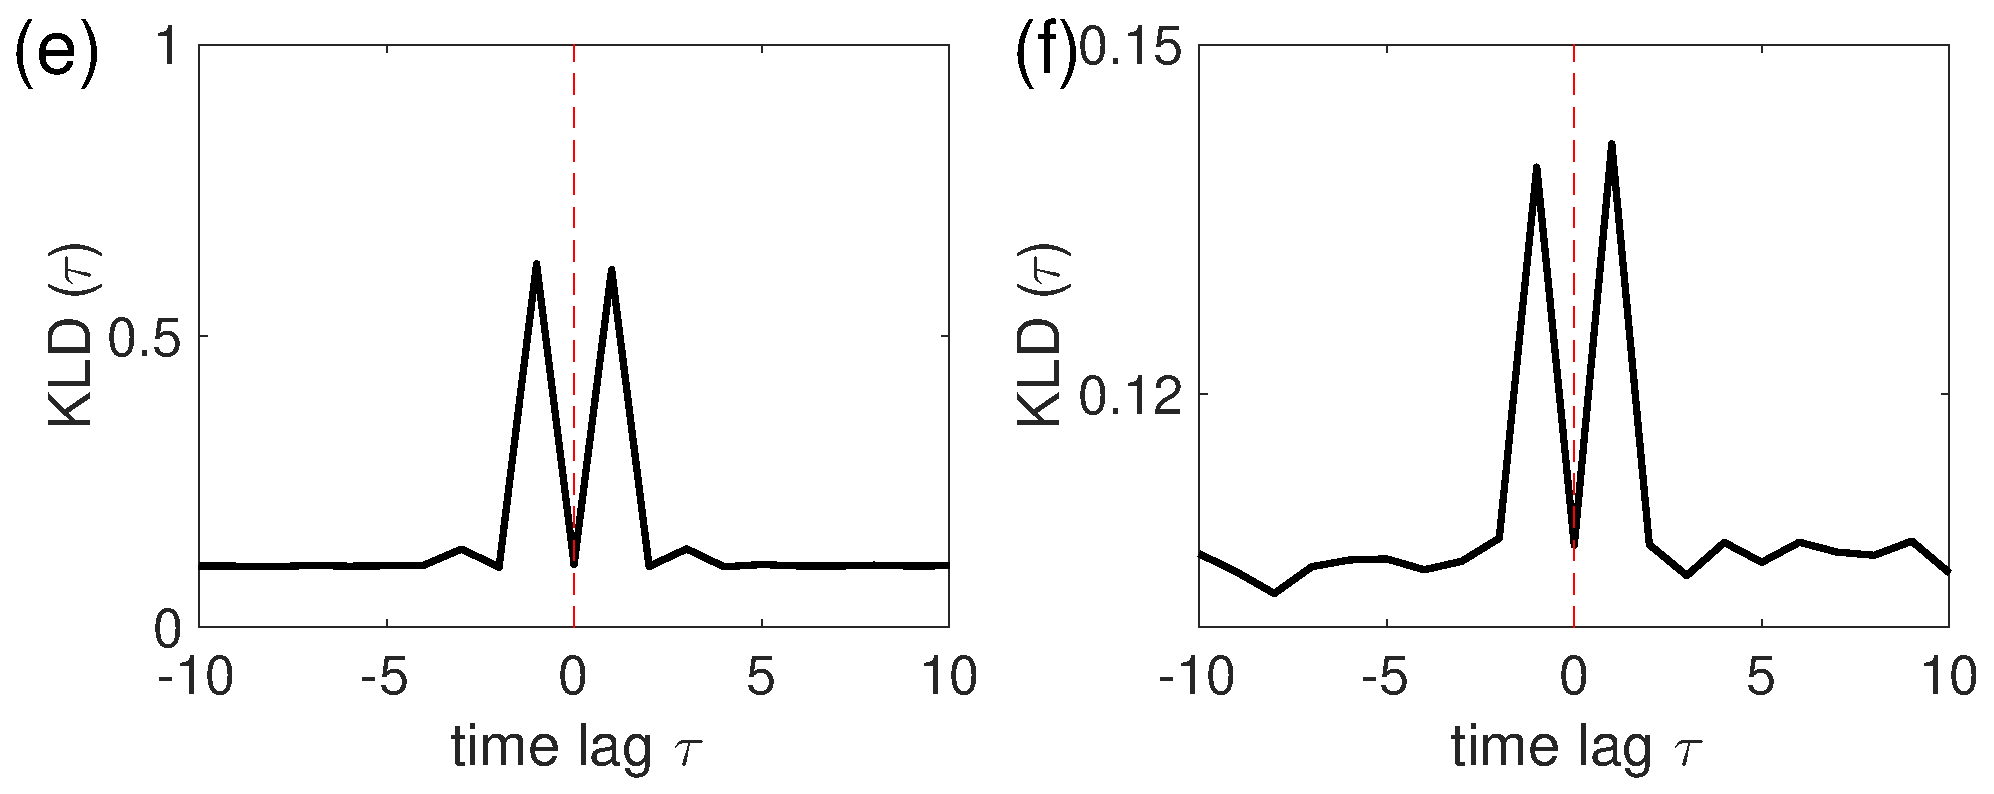
\includegraphics[width=\columnwidth]{KL_D.eps}
\caption{(Color online) Same as in Fig.~\ref{fig:stdHeqB} but for Eq. (11).  {\color{red}Note that the error bars have been enlarged by 1000 times.} \label{fig:stdHeqD}}
\end{figure}

\begin{figure}
	\centering
	\includegraphics[width=0.5\columnwidth]{/Users/yongzou/Documents/TimeSeries_Network/OrderPatternPermutation/RuanFiguresPlot2018/errorbarE_E.eps}
%	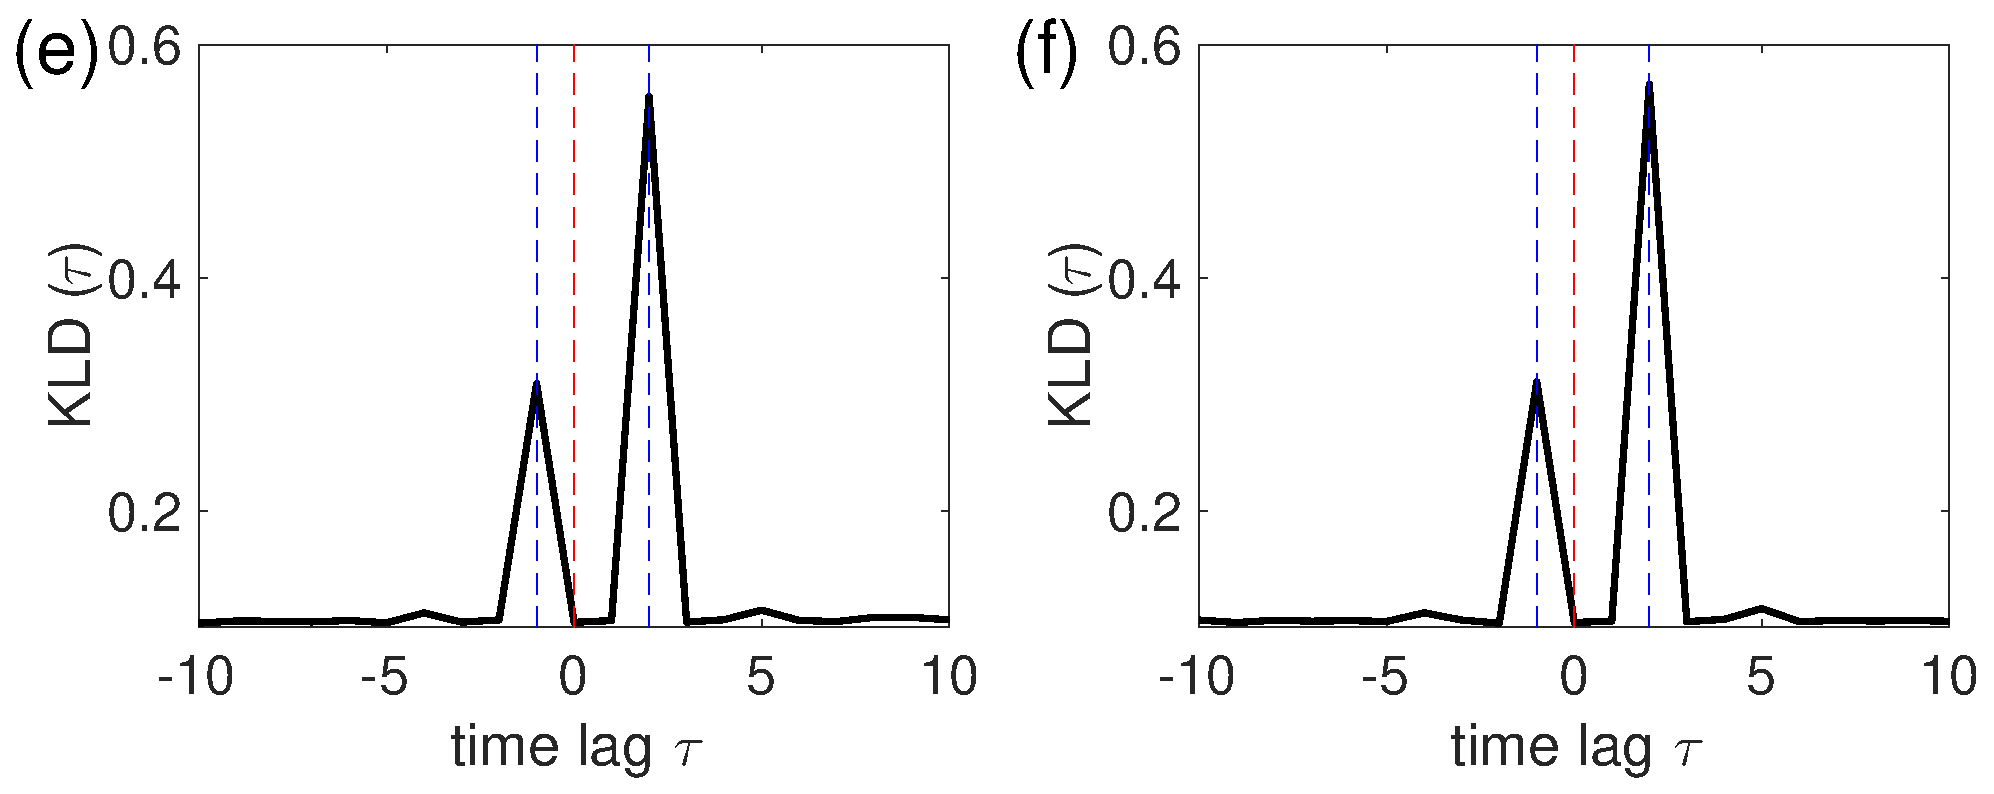
\includegraphics[width=\columnwidth]{KL_E.eps}
\caption{(Color online) Same as in Fig.~\ref{fig:stdHeqD} but for Eq. (12). The two employed delays of $\tau = -1$ and $\tau = 2$ are additionally highlighted by vertical blue dashed lines. {\color{red}Note that the error bars have been enlarged by 1000 times.}\label{fig:stdHeqE}}
\end{figure}



\noindent {\sf 2- Figures 9 and 10 show results only for KLD measure. Why not for all quantifiers? 
Figures 9 and 10 also show that KLD is a reliable quantifier only for time series larger than 10000. Such a result is consistent for both systems considered in the figures. 
Fig. 11 shows results for an experimental situation where the available data size is on the same order (10000). So the results must be corroborated at least using other quantifiers. A sentence discussing it will be also appreciated. 
}

\begin{center}
\begin{minipage}[c]{0.9\textwidth}
We have included the discussion as suggested, in particular the results are reliable if time series length larger than 10000. 
\end{minipage}
\end{center}



\noindent
{\sf 1- Please, provide References for the sentences: 

" In general, temperature records like those used here are characterized by some irregular alternation between colder and warmer phases due to large-scale atmospheric patterns (corresponding to high and low pressure centers, respectively), which in the case of western-to- central Europe travel in the majority of situations in eastward direction." 


"This coupling delay is reasonable since temperature variations in Oxford arising from general atmospheric circulation patterns are typically propagated eastward and reach Vienna about 1to 2 days later, which corresponds to the average propagation speed of frontal systems in the northern mid-latitudes west-wind zone."}

\begin{center}
\begin{minipage}[c]{0.9\textwidth}
Reik, please provide the references for the above two statements. 
\end{minipage}
\end{center}


\end{document}
